\documentclass[12pt,letterpaper, onecolumn]{exam}
\usepackage{amsmath}
\usepackage{amssymb}
\usepackage{multicol}
\usepackage{graphicx}
\usepackage{pgfplots}
\usepackage{amsthm}
\usepackage[lmargin=71pt, tmargin=1.2in]{geometry}  %For centering solution box
% \chead{\hline} % Un-comment to draw line below header
\thispagestyle{empty}   %For removing header/footer from page 1

\begin{document}

\begingroup  
    \centering
    \LARGE Fonctions quadratiques, Corrigé\\[0.5em]
    \large Série 1, 26 octobre 2021\\
    \large 4CPT-2M\par
\endgroup
\rule{\textwidth}{0.4pt}
\begin{enumerate}
    \item Écrire ces fonctions sous leur forme générale\\
    On cherche à écrire les fonctions sous la forme $f(x)=ax^2+bx+c$
    \begin{enumerate}
        \item $f(x)=\dfrac{(x-2)^2+3}{2} = \frac{1}{2}x^2 -2x + \frac{7}{2}$
        \item $f(x)=x^2+x(x-1)-x(x+1)-4 = x^2 -2x -4$
        \item $f(x)=\dfrac{(x-1)^3+1}{x} = x^2 -3x +3$
        \item $f(x)=\dfrac{(x+6)(x+10)}{4} = \frac{1}{4}x^2 +4x + 15$
    \end{enumerate}
    Dans la $1^{ère}$ version la fonction (c) était légèrement différente :
    \[f(x)=\dfrac{(x-1)^3-1}{x} = x^2 -3x +3 -\dfrac{2}{x}\]
    Ce n'est pas une fonction quadratique, vu le terme $\dfrac{2}{x}$ à la fin
    \item Écrire ces fonctions sous leur forme canonique et donnez les coordonnées du sommet\\
    On cherche à écrire les fonctions sous la forme $f(x)=a(x-m)^2+n$ avec $m=\dfrac{-b}{2a}$ et $n=\dfrac{4ac-b^2}{4a}$
    \begin{enumerate}
        \item $f(x)=x(x-1) = (x-\frac{1}{2})^2-\frac{1}{4}, \quad S=(\frac{1}{2};-\frac{1}{4})$
        \item $f(x)=2x^2+2x-1 = 2(x+\frac{1}{2})^2-\frac{3}{2}, \quad S=(-\frac{1}{2};-\frac{3}{2})$
        \item $f(x)=x^2-2x+2 = (x-1)^2+1, \quad S=(1;1)$
        \item $f(x)=\frac{1}{2}(x+1)(x+3) = \frac{1}{2}(x+2)^2-\frac{1}{2}, \quad S=(-2;-\frac{1}{2})$
    \end{enumerate}
    \item Écrire ces fonctions sous leur forme factorisée, et donnez le ou les zéro(s)\\
    On cherche à écrire ces fonctions sous la forme $f(x)=a(x-x_1)(x-x_2)$ en utilisant la formule de Viète pour trouver les zéros $x_1$ et $x_2$
    \begin{enumerate}
        \item $f(x)=3x^2+12x+12 = 3(x+2)^2, \quad x_1=x_2=-2$
        \item $f(x)=\frac{-1}{4}(x-5)^2+2 = -\frac{1}{4}(x-5-2 \sqrt{2})(x-5+2\sqrt{2}),\\ \quad x_1=5-2\sqrt{2}, \quad x_2=5+2\sqrt{2}$
        \item $f(x)=(x-\frac{1}{2})^2-1 = (x+\frac{1}{2})(x-\frac{3}{2}), \quad x_1=-\frac{1}{2}, \quad x_2=\frac{3}{2}$
        \item $f(x)=\dfrac{x^2-6x+9}{3}=\frac{1}{3}(x-3)^2, \quad x_1=x_2=3$
    \end{enumerate}
    \item Trouvez les zéros, les coordonnées du sommet ainsi que l'ordonnée à l'origine des fonctions suivantes, puis tracez leur graphe
    \begin{enumerate}
        \item $f(x)=\dfrac{x^2}{3}+x-\frac{4}{3}$
            \[x_1=-\frac{3}{2} - \frac{5}{2} \quad x_2=-\frac{3}{2} + \frac{5}{2} \quad S=\Big(-\frac{3}{2}; -\frac{31}{12}\Big) \quad y_0= -\frac{4}{3}\]
            \begin{center}
            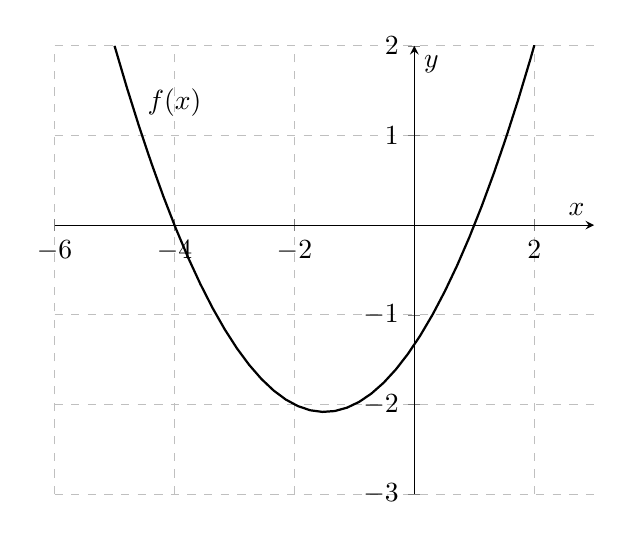
\begin{tikzpicture}
            \begin{axis}[
                xlabel style = {above right},
                ylabel style = {above left},
                xmin=-6, xmax=3,
                ymin=-3, ymax=2,
                xlabel={$x$},
                ylabel={$y$},
                axis lines=center,
                xmajorgrids=true,
                ymajorgrids=true,
                grid style=dashed,
                samples=50
            ]
            \addplot[black, thick] (x,x^2/3+x-4/3);
            \node[label={90:{$f(x)$}}] at (axis cs:-4,1) {};
            \end{axis}
            \end{tikzpicture}
            \end{center}
        \item $f(x)=(x-2)^2+d \qquad$ avec $ d\in\{-1, 0, 1\}$\\[0.5em]
        Solutions générales :
        \[x_1=2-\sqrt{-d} \quad x_2=2+\sqrt{-d} \quad S=(2;d) \quad y_0=4+d\]
        Pour $d=0$ on a $x_1=x_2$, et pour $d=1$ il n'existe pas de zéro
        \begin{center}
            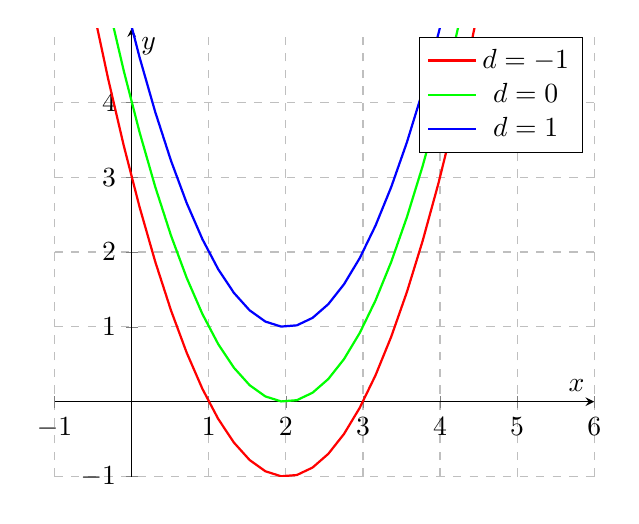
\begin{tikzpicture}
            \begin{axis}[
                xlabel style = {above right},
                ylabel style = {above left},
                xmin=-1, xmax=6,
                ymin=-1, ymax=4.99,
                xlabel={$x$},
                ylabel={$y$},
                axis lines=center,
                xmajorgrids=true,
                ymajorgrids=true,
                grid style=dashed,
                samples=50
            ]
            \addplot[red, thick] (x,x^2-4*x+3);
            \addlegendentry{\(d=-1\)}
            \addplot[green, thick] (x,x^2-4*x+4);
            \addlegendentry{\(d=0\)}
            \addplot[blue, thick] (x,x^2-4*x+5);
            \addlegendentry{\(d=1\)}
            \end{axis}
            \end{tikzpicture}
            \end{center}
    \end{enumerate}
\end{enumerate}
\end{document}